\chapter{Processi e metodologie}
\label{cap:processi-metodologie}

\intro{In questa sezione viene illustrato l’approccio organizzativo adottato per il progetto, includendo le strategie implementate per automatizzare i processi.}

\section{Modello di sviluppo}

\par L’organizzazione del lavoro è stata gestita tramite la piattaforma Jira, utilizzando un template \textit{Kanban} semplificato. Questo modello fornisce una \textit{timeline}, una \textit{board} suddivisa nelle etichette “Da completare”, “In corso” e “Completato” (analogamente a Trello), un calendario e una \textit{dashboard} per monitorare l’integrazione con \gls{github}. Il progetto è stato suddiviso in tre \textit{epic}, o macro-fasi (analisi, sviluppo, validazione), ciascuna delle quali si è conclusa con il rilascio di un prodotto. Ogni rilascio di documentazione o software è stato associato a una specifica \textit{milestone}. Il tempo dedicato ai tre \textit{epic} è stato ulteriormente articolato in periodi settimanali (simili agli \textit{sprint} della metodologia \textit{agile}). Questo approccio ha permesso di mantenere un rapporto costante con la Proponente; al termine di ogni periodo è stato fornito un aggiornamento sullo stato di avanzamento, in presenza o da remoto (tramite comunicazione via e-mail), e sono state pianificate le attività successive. La priorità delle attività è stata concordata settimanalmente con la Proponente, così da definire un elenco ordinato (simile a un \textit{backlog}) di \textit{task} da completare entro la fine dell’iterazione.

\section{Workflow GitHub}

\par Per gestire lo sviluppo, ho adottato una struttura basata su due \textit{branch} principali: \textit{main} e \textit{develop}. Il \textit{branch main} registra la cronologia dei rilasci e contiene codice stabile, pronto per la produzione, mentre \textit{develop} rappresenta la linea di sviluppo principale. A ciascuna funzionalità da implementare è associato un \textit{branch} dedicato, contraddistinto dal prefisso \textit{feature/}, che ne accompagna lo sviluppo fino all’integrazione in un ramo condiviso. Quando una funzionalità risulta completa o pronta per l’integrazione, viene sottoposta a revisione tramite l’apertura di una \textit{pull request}, che può essere arricchita con commenti, etichette, \textit{issue} e \textit{milestone}.

\vspace{10pt}
\par\noindent Questo flusso di lavoro è riconducibile al modello \textit{Gitflow}, introdotto da Vincent Driessen nel 2010. Nell’ambito del progetto di stage, il modello \textit{Gitflow} non è stato applicato in modo rigido, ma ibridato con alcuni principi dello sviluppo \textit{trunk-based}. Idealmente, \textit{Gitflow} prevede \textit{branch} isolati e di lunga durata, mentre l’approccio \textit{trunk-based} favorisce aggiornamenti piccoli e frequenti, anche in assenza del completamento di una funzionalità, sfruttando appieno il potenziale della \textit{continuous integration}.

\vspace{10pt}
\par\noindent Per avviare il rilascio di una nuova versione, \textit{Gitflow} prevede la creazione di un \textit{branch} con il prefisso \textit{release/}. Il rilascio vero e proprio si concretizza con l’integrazione nel \textit{branch main}, che viene contrassegnato con un numero di versione. La versione può essere etichettata come “latest” oppure “pre-release”, qualora non sia ancora pronta per l’ambiente di produzione. Al termine del rilascio, i due \textit{branch} principali, \textit{main} e \textit{develop}, devono essere riallineati.

\section{Workflow Jira}

\par Prima di creare un branch su \gls{github}, a ciascuna funzionalità viene associato un \textit{ticket}, che può essere arricchito con commenti, etichette, date di inizio e fine, ed eventuali sotto-ticket. La creazione del \textit{branch} può avvenire direttamente da Jira, così da garantire un collegamento automatico con il relativo \textit{ticket}. In alternativa, il collegamento tra un \textit{ticket} e un \textit{branch}, un \textit{commit} o una \textit{pull request} può essere stabilito inserendo l’ID del \textit{ticket} come commento. Se l’ID viene racchiuso tra parentesi quadre (es. [ID]) all’interno della sezione commenti di una \textit{pull request}, il \textit{bot} di Jira genera automaticamente un collegamento ipertestuale al progetto.

\section{Automatizzazione dei processi}

\par Ho configurato un \textit{workflow}, tramite \textit{GitHub Actions}, che si attiva a ogni apertura, aggiornamento o chiusura di una \textit{pull request}. Il \textit{workflow}, scritto in \gls{yaml}, avvia due \textit{job} principali: l’esecuzione dei test automatizzati e il monitoraggio della \textit{code coverage}. Per i test è stato adottato il \textit{framework} Jest, che produce automaticamente un report sulla copertura del codice. Il report viene inviato a Codecov, che aggiorna la \textit{dashboard} del progetto, genera un \textit{badge} di stato e pubblica un riepilogo nei commenti della \textit{pull request}. Il superamento dei test e il mantenimento della copertura (rispetto alla versione precedente) rappresentano condizioni necessarie per procedere con il \textit{merge}. Questo approccio promuove la \textit{continuous integration} e fornisce una valutazione oggettiva della qualità del codice.

\vspace{10pt}
\par\noindent Su Jira ho definito tre regole di automazione:
\begin{itemize}
  \item \textbf{PR\_merged}: si attiva quando viene eseguito il \textit{merge} di una \textit{pull request} e sposta i \textit{ticket} collegati dallo stato corrente a “Completato”;
  \item \textbf{TICKET\_closed}: si attiva quando tutti i \textit{ticket} subordinati risultano completati e sposta l'elemento principale dallo stato corrente a “Completato”;
  \item \textbf{TICKET\_reopened}: si attiva quando un \textit{ticket} subordinato viene (ri)aperto e sposta l’elemento principale dallo stato “Completato” a “In corso”.
\end{itemize}

\begin{figure}[H] 
  \centering 
  \fbox{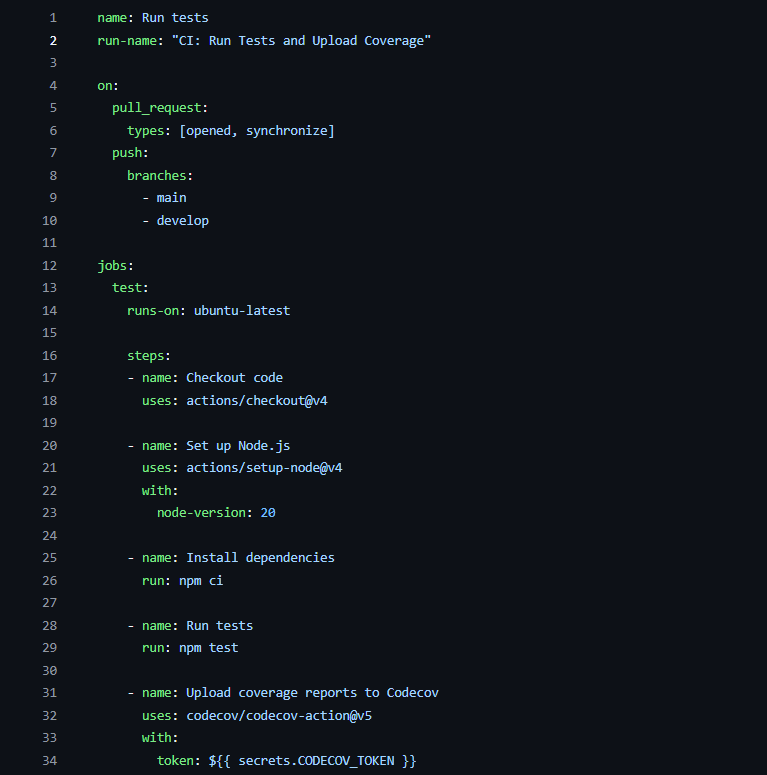
\includegraphics[width=0.9\textwidth]{processi/workflow.png}}
  \caption{Workflow YAML per continuous integration}
\end{figure}